% Options for packages loaded elsewhere
\PassOptionsToPackage{unicode}{hyperref}
\PassOptionsToPackage{hyphens}{url}
\PassOptionsToPackage{dvipsnames,svgnames,x11names}{xcolor}
%
\documentclass[
  letterpaper,
  DIV=11,
  numbers=noendperiod]{scrartcl}

\usepackage{amsmath,amssymb}
\usepackage{iftex}
\ifPDFTeX
  \usepackage[T1]{fontenc}
  \usepackage[utf8]{inputenc}
  \usepackage{textcomp} % provide euro and other symbols
\else % if luatex or xetex
  \usepackage{unicode-math}
  \defaultfontfeatures{Scale=MatchLowercase}
  \defaultfontfeatures[\rmfamily]{Ligatures=TeX,Scale=1}
\fi
\usepackage{lmodern}
\ifPDFTeX\else  
    % xetex/luatex font selection
\fi
% Use upquote if available, for straight quotes in verbatim environments
\IfFileExists{upquote.sty}{\usepackage{upquote}}{}
\IfFileExists{microtype.sty}{% use microtype if available
  \usepackage[]{microtype}
  \UseMicrotypeSet[protrusion]{basicmath} % disable protrusion for tt fonts
}{}
\makeatletter
\@ifundefined{KOMAClassName}{% if non-KOMA class
  \IfFileExists{parskip.sty}{%
    \usepackage{parskip}
  }{% else
    \setlength{\parindent}{0pt}
    \setlength{\parskip}{6pt plus 2pt minus 1pt}}
}{% if KOMA class
  \KOMAoptions{parskip=half}}
\makeatother
\usepackage{xcolor}
\setlength{\emergencystretch}{3em} % prevent overfull lines
\setcounter{secnumdepth}{-\maxdimen} % remove section numbering
% Make \paragraph and \subparagraph free-standing
\makeatletter
\ifx\paragraph\undefined\else
  \let\oldparagraph\paragraph
  \renewcommand{\paragraph}{
    \@ifstar
      \xxxParagraphStar
      \xxxParagraphNoStar
  }
  \newcommand{\xxxParagraphStar}[1]{\oldparagraph*{#1}\mbox{}}
  \newcommand{\xxxParagraphNoStar}[1]{\oldparagraph{#1}\mbox{}}
\fi
\ifx\subparagraph\undefined\else
  \let\oldsubparagraph\subparagraph
  \renewcommand{\subparagraph}{
    \@ifstar
      \xxxSubParagraphStar
      \xxxSubParagraphNoStar
  }
  \newcommand{\xxxSubParagraphStar}[1]{\oldsubparagraph*{#1}\mbox{}}
  \newcommand{\xxxSubParagraphNoStar}[1]{\oldsubparagraph{#1}\mbox{}}
\fi
\makeatother

\usepackage{color}
\usepackage{fancyvrb}
\newcommand{\VerbBar}{|}
\newcommand{\VERB}{\Verb[commandchars=\\\{\}]}
\DefineVerbatimEnvironment{Highlighting}{Verbatim}{commandchars=\\\{\}}
% Add ',fontsize=\small' for more characters per line
\usepackage{framed}
\definecolor{shadecolor}{RGB}{241,243,245}
\newenvironment{Shaded}{\begin{snugshade}}{\end{snugshade}}
\newcommand{\AlertTok}[1]{\textcolor[rgb]{0.68,0.00,0.00}{#1}}
\newcommand{\AnnotationTok}[1]{\textcolor[rgb]{0.37,0.37,0.37}{#1}}
\newcommand{\AttributeTok}[1]{\textcolor[rgb]{0.40,0.45,0.13}{#1}}
\newcommand{\BaseNTok}[1]{\textcolor[rgb]{0.68,0.00,0.00}{#1}}
\newcommand{\BuiltInTok}[1]{\textcolor[rgb]{0.00,0.23,0.31}{#1}}
\newcommand{\CharTok}[1]{\textcolor[rgb]{0.13,0.47,0.30}{#1}}
\newcommand{\CommentTok}[1]{\textcolor[rgb]{0.37,0.37,0.37}{#1}}
\newcommand{\CommentVarTok}[1]{\textcolor[rgb]{0.37,0.37,0.37}{\textit{#1}}}
\newcommand{\ConstantTok}[1]{\textcolor[rgb]{0.56,0.35,0.01}{#1}}
\newcommand{\ControlFlowTok}[1]{\textcolor[rgb]{0.00,0.23,0.31}{\textbf{#1}}}
\newcommand{\DataTypeTok}[1]{\textcolor[rgb]{0.68,0.00,0.00}{#1}}
\newcommand{\DecValTok}[1]{\textcolor[rgb]{0.68,0.00,0.00}{#1}}
\newcommand{\DocumentationTok}[1]{\textcolor[rgb]{0.37,0.37,0.37}{\textit{#1}}}
\newcommand{\ErrorTok}[1]{\textcolor[rgb]{0.68,0.00,0.00}{#1}}
\newcommand{\ExtensionTok}[1]{\textcolor[rgb]{0.00,0.23,0.31}{#1}}
\newcommand{\FloatTok}[1]{\textcolor[rgb]{0.68,0.00,0.00}{#1}}
\newcommand{\FunctionTok}[1]{\textcolor[rgb]{0.28,0.35,0.67}{#1}}
\newcommand{\ImportTok}[1]{\textcolor[rgb]{0.00,0.46,0.62}{#1}}
\newcommand{\InformationTok}[1]{\textcolor[rgb]{0.37,0.37,0.37}{#1}}
\newcommand{\KeywordTok}[1]{\textcolor[rgb]{0.00,0.23,0.31}{\textbf{#1}}}
\newcommand{\NormalTok}[1]{\textcolor[rgb]{0.00,0.23,0.31}{#1}}
\newcommand{\OperatorTok}[1]{\textcolor[rgb]{0.37,0.37,0.37}{#1}}
\newcommand{\OtherTok}[1]{\textcolor[rgb]{0.00,0.23,0.31}{#1}}
\newcommand{\PreprocessorTok}[1]{\textcolor[rgb]{0.68,0.00,0.00}{#1}}
\newcommand{\RegionMarkerTok}[1]{\textcolor[rgb]{0.00,0.23,0.31}{#1}}
\newcommand{\SpecialCharTok}[1]{\textcolor[rgb]{0.37,0.37,0.37}{#1}}
\newcommand{\SpecialStringTok}[1]{\textcolor[rgb]{0.13,0.47,0.30}{#1}}
\newcommand{\StringTok}[1]{\textcolor[rgb]{0.13,0.47,0.30}{#1}}
\newcommand{\VariableTok}[1]{\textcolor[rgb]{0.07,0.07,0.07}{#1}}
\newcommand{\VerbatimStringTok}[1]{\textcolor[rgb]{0.13,0.47,0.30}{#1}}
\newcommand{\WarningTok}[1]{\textcolor[rgb]{0.37,0.37,0.37}{\textit{#1}}}

\providecommand{\tightlist}{%
  \setlength{\itemsep}{0pt}\setlength{\parskip}{0pt}}\usepackage{longtable,booktabs,array}
\usepackage{calc} % for calculating minipage widths
% Correct order of tables after \paragraph or \subparagraph
\usepackage{etoolbox}
\makeatletter
\patchcmd\longtable{\par}{\if@noskipsec\mbox{}\fi\par}{}{}
\makeatother
% Allow footnotes in longtable head/foot
\IfFileExists{footnotehyper.sty}{\usepackage{footnotehyper}}{\usepackage{footnote}}
\makesavenoteenv{longtable}
\usepackage{graphicx}
\makeatletter
\def\maxwidth{\ifdim\Gin@nat@width>\linewidth\linewidth\else\Gin@nat@width\fi}
\def\maxheight{\ifdim\Gin@nat@height>\textheight\textheight\else\Gin@nat@height\fi}
\makeatother
% Scale images if necessary, so that they will not overflow the page
% margins by default, and it is still possible to overwrite the defaults
% using explicit options in \includegraphics[width, height, ...]{}
\setkeys{Gin}{width=\maxwidth,height=\maxheight,keepaspectratio}
% Set default figure placement to htbp
\makeatletter
\def\fps@figure{htbp}
\makeatother

\KOMAoption{captions}{tableheading}
\makeatletter
\@ifpackageloaded{caption}{}{\usepackage{caption}}
\AtBeginDocument{%
\ifdefined\contentsname
  \renewcommand*\contentsname{Table of contents}
\else
  \newcommand\contentsname{Table of contents}
\fi
\ifdefined\listfigurename
  \renewcommand*\listfigurename{List of Figures}
\else
  \newcommand\listfigurename{List of Figures}
\fi
\ifdefined\listtablename
  \renewcommand*\listtablename{List of Tables}
\else
  \newcommand\listtablename{List of Tables}
\fi
\ifdefined\figurename
  \renewcommand*\figurename{Figure}
\else
  \newcommand\figurename{Figure}
\fi
\ifdefined\tablename
  \renewcommand*\tablename{Table}
\else
  \newcommand\tablename{Table}
\fi
}
\@ifpackageloaded{float}{}{\usepackage{float}}
\floatstyle{ruled}
\@ifundefined{c@chapter}{\newfloat{codelisting}{h}{lop}}{\newfloat{codelisting}{h}{lop}[chapter]}
\floatname{codelisting}{Listing}
\newcommand*\listoflistings{\listof{codelisting}{List of Listings}}
\makeatother
\makeatletter
\makeatother
\makeatletter
\@ifpackageloaded{caption}{}{\usepackage{caption}}
\@ifpackageloaded{subcaption}{}{\usepackage{subcaption}}
\makeatother
\ifLuaTeX
  \usepackage{selnolig}  % disable illegal ligatures
\fi
\usepackage{bookmark}

\IfFileExists{xurl.sty}{\usepackage{xurl}}{} % add URL line breaks if available
\urlstyle{same} % disable monospaced font for URLs
\hypersetup{
  pdftitle={Métodos numéricos},
  colorlinks=true,
  linkcolor={blue},
  filecolor={Maroon},
  citecolor={Blue},
  urlcolor={Blue},
  pdfcreator={LaTeX via pandoc}}

\title{Métodos numéricos}
\author{}
\date{}

\begin{document}
\maketitle

\begin{enumerate}
\def\labelenumi{\arabic{enumi}.}
\tightlist
\item
  Para cada uno de los siguientes sistemas lineales, obtenga, de ser
  posible, una solución con métodos gráficos.
\end{enumerate}

\begin{enumerate}
\def\labelenumi{\alph{enumi}.}
\tightlist
\item
  \(x_1 + 2x_2 = 0\), \(x_1 - x_2 = 0\)
\end{enumerate}

\begin{Shaded}
\begin{Highlighting}[]
\ImportTok{from}\NormalTok{ src }\ImportTok{import}\NormalTok{ plot\_system}
\NormalTok{a1, b1, c1 }\OperatorTok{=} \DecValTok{1}\NormalTok{, }\DecValTok{2}\NormalTok{, }\DecValTok{0}
\NormalTok{a2, b2, c2 }\OperatorTok{=} \DecValTok{1}\NormalTok{, }\OperatorTok{{-}}\DecValTok{1}\NormalTok{, }\DecValTok{0}
\NormalTok{plot\_system(a1, b1, c1, a2, b2, c2)}
\end{Highlighting}
\end{Shaded}

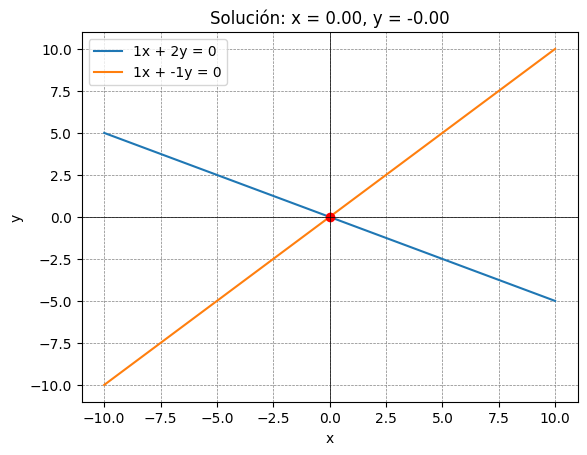
\includegraphics{tarea9_files/figure-pdf/cell-2-output-1.png}

\begin{enumerate}
\def\labelenumi{\alph{enumi}.}
\setcounter{enumi}{1}
\tightlist
\item
  \(x_1 + 2x_2 = 3\), \(-2x_1 - 4x_2 = 6\)
\end{enumerate}

\begin{Shaded}
\begin{Highlighting}[]
\ImportTok{from}\NormalTok{ src }\ImportTok{import}\NormalTok{ plot\_system}
\ImportTok{from}\NormalTok{ src }\ImportTok{import}\NormalTok{ eliminacion\_gaussiana}

\NormalTok{a1, b1, c1 }\OperatorTok{=} \DecValTok{1}\NormalTok{, }\DecValTok{2}\NormalTok{, }\DecValTok{3}
\NormalTok{a2, b2, c2 }\OperatorTok{=} \OperatorTok{{-}}\DecValTok{2}\NormalTok{, }\OperatorTok{{-}}\DecValTok{4}\NormalTok{, }\DecValTok{6}
\NormalTok{plot\_system(a1, b1, c1, a2, b2, c2)}
\end{Highlighting}
\end{Shaded}

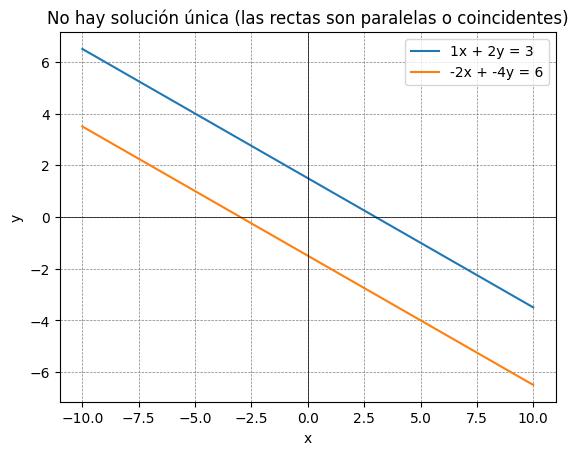
\includegraphics{tarea9_files/figure-pdf/cell-3-output-1.png}

\begin{enumerate}
\def\labelenumi{\alph{enumi}.}
\setcounter{enumi}{2}
\tightlist
\item
  \(2x_1 + x_2 = -1\), \(x_1 - x_2 = 2\), \(x_1-3x_2=5\)
\end{enumerate}

Se espera que sea una ecuacion consistente para esto, la resolución
puede darse mediante la reducción Gaussiana, o propiamente implementando
una función de resolución mas compleja en relacion a la propuesta para
los demás ejercicios.

\begin{enumerate}
\def\labelenumi{\alph{enumi}.}
\setcounter{enumi}{3}
\tightlist
\item
  \(2x_1 + x_2 + x_3 = 1\), \(2x_1 + 4x_2 - x_3 = -2\)
\end{enumerate}

Dado que en el sistema se presentan mas variables que ecuaciones, la
solución de la misma es indefinida.

\begin{enumerate}
\def\labelenumi{\arabic{enumi}.}
\setcounter{enumi}{1}
\tightlist
\item
  Utilice la eliminación gaussiana con sustitución hacia atrás y
  aritmética de dos d;igitos para resolver los siguientes sistemas
  lineales.
\end{enumerate}

\begin{enumerate}
\def\labelenumi{\alph{enumi}.}
\tightlist
\item
  \(-x_1 + 4x_2 + x_3 = 8\),
  \(\frac{5}{3}x_1 + \frac{2}{3}x_2 +\frac{2}{3}x_3 = 1\),
  \(2x_1 + x_2 +4x_3 = 11\)
\end{enumerate}

\begin{Shaded}
\begin{Highlighting}[]
\NormalTok{A }\OperatorTok{=}\NormalTok{ [[}\OperatorTok{{-}}\DecValTok{1}\NormalTok{,}\DecValTok{4}\NormalTok{,}\DecValTok{1}\NormalTok{,}\DecValTok{8}\NormalTok{],[}\FloatTok{1.67}\NormalTok{,}\FloatTok{0.67}\NormalTok{,}\FloatTok{0.67}\NormalTok{,}\DecValTok{1}\NormalTok{],[}\DecValTok{2}\NormalTok{,}\DecValTok{1}\NormalTok{,}\DecValTok{4}\NormalTok{,}\FloatTok{11.}\NormalTok{]]}
\NormalTok{eliminacion\_gaussiana(A)}
\end{Highlighting}
\end{Shaded}

\begin{verbatim}
[07-21 17:49:48][INFO] 
[[-1.    4.    1.    8.  ]
 [ 0.    7.35  2.34 14.36]
 [ 0.    9.    6.   27.  ]]
[07-21 17:49:48][INFO] 
[[-1.          4.          1.          8.        ]
 [ 0.          7.35        2.34       14.36      ]
 [ 0.          0.          3.13469388  9.41632653]]
\end{verbatim}

\begin{verbatim}
array([-1.00651042,  0.99739583,  3.00390625])
\end{verbatim}

\begin{enumerate}
\def\labelenumi{\alph{enumi}.}
\setcounter{enumi}{1}
\tightlist
\item
  \(4x_1 + 2x_2 - x_3 = -5\),
  \(\frac{1}{9}x_1 + \frac{1}{9}x_2 -\frac{1}{3}x_3 = -1\),
  \(x_1 + 4x_2 +2x_3 = 9\)
\end{enumerate}

\begin{Shaded}
\begin{Highlighting}[]
\NormalTok{B }\OperatorTok{=}\NormalTok{ [[}\DecValTok{4}\NormalTok{,}\DecValTok{2}\NormalTok{,}\OperatorTok{{-}}\DecValTok{1}\NormalTok{,}\OperatorTok{{-}}\DecValTok{5}\NormalTok{],[}\FloatTok{0.11}\NormalTok{,}\FloatTok{0.11}\NormalTok{,}\OperatorTok{{-}}\FloatTok{0.33}\NormalTok{,}\OperatorTok{{-}}\DecValTok{1}\NormalTok{],[}\DecValTok{1}\NormalTok{,}\DecValTok{4}\NormalTok{,}\DecValTok{2}\NormalTok{,}\DecValTok{9}\NormalTok{]]}
\NormalTok{eliminacion\_gaussiana(B)}
\end{Highlighting}
\end{Shaded}

\begin{verbatim}
[07-21 17:55:56][INFO] 
[[ 0.11        0.11       -0.33       -1.        ]
 [ 0.         -2.         11.         31.36363636]
 [ 0.          3.          5.         18.09090909]]
[07-21 17:55:56][INFO] 
[[ 0.11        0.11       -0.33       -1.        ]
 [ 0.         -2.         11.         31.36363636]
 [ 0.          0.         21.5        65.13636364]]
\end{verbatim}

\begin{verbatim}
array([-0.98308668,  0.98097252,  3.02959831])
\end{verbatim}

\begin{enumerate}
\def\labelenumi{\arabic{enumi}.}
\setcounter{enumi}{2}
\tightlist
\item
  Utilice el algoritmo de eliminación guassiana para resolver, de ser
  posible, los siguientes sistemas lineales, y determine si se necesitan
  intercambios de fila.
\end{enumerate}

\begin{enumerate}
\def\labelenumi{\alph{enumi}.}
\tightlist
\item
  \(x_1 - x_2 +3 x_3 = 2\), \(3x_1 -3x_2 +x_3 = -1\), \(x_1 + x_2 = 3\)
\end{enumerate}

\begin{Shaded}
\begin{Highlighting}[]
\NormalTok{A }\OperatorTok{=}\NormalTok{ [[}\DecValTok{1}\NormalTok{,}\OperatorTok{{-}}\DecValTok{1}\NormalTok{,}\DecValTok{3}\NormalTok{,}\DecValTok{2}\NormalTok{],[}\DecValTok{3}\NormalTok{,}\OperatorTok{{-}}\DecValTok{3}\NormalTok{,}\DecValTok{1}\NormalTok{,}\OperatorTok{{-}}\DecValTok{1}\NormalTok{],[}\DecValTok{1}\NormalTok{,}\DecValTok{1}\NormalTok{,}\DecValTok{0}\NormalTok{,}\FloatTok{3.}\NormalTok{]]}
\NormalTok{eliminacion\_gaussiana(A)}
\end{Highlighting}
\end{Shaded}

\begin{verbatim}
[07-21 17:57:42][INFO] 
[[ 1. -1.  3.  2.]
 [ 0.  0. -8. -7.]
 [ 0.  2. -3.  1.]]
[07-21 17:57:42][INFO] 
[[ 1. -1.  3.  2.]
 [ 0.  2. -3.  1.]
 [ 0.  0. -8. -7.]]
\end{verbatim}

\begin{verbatim}
array([1.1875, 1.8125, 0.875 ])
\end{verbatim}

\begin{enumerate}
\def\labelenumi{\alph{enumi}.}
\setcounter{enumi}{1}
\tightlist
\item
  \(2x_1 -1.5 x_2 +3 x_3 = 1\), \(-x_1 +2x_3 = 3\),
  \(4x_1 -4.5 x_2+5x_3 = 1\)
\end{enumerate}

\begin{Shaded}
\begin{Highlighting}[]
\NormalTok{B }\OperatorTok{=}\NormalTok{ [[}\DecValTok{2}\NormalTok{,}\OperatorTok{{-}}\FloatTok{1.5}\NormalTok{,}\DecValTok{3}\NormalTok{,}\DecValTok{1}\NormalTok{],[}\OperatorTok{{-}}\DecValTok{1}\NormalTok{,}\DecValTok{0}\NormalTok{,}\DecValTok{2}\NormalTok{,}\DecValTok{3}\NormalTok{],[}\DecValTok{4}\NormalTok{,}\OperatorTok{{-}}\FloatTok{4.5}\NormalTok{,}\DecValTok{5}\NormalTok{,}\FloatTok{1.}\NormalTok{]]}
\NormalTok{eliminacion\_gaussiana(B)}
\end{Highlighting}
\end{Shaded}

\begin{verbatim}
[07-21 18:02:42][INFO] 
[[-1.   0.   2.   3. ]
 [ 0.  -1.5  7.   7. ]
 [ 0.  -4.5 13.  13. ]]
[07-21 18:02:42][INFO] 
[[-1.   0.   2.   3. ]
 [ 0.  -1.5  7.   7. ]
 [ 0.   0.  -8.  -8. ]]
\end{verbatim}

\begin{verbatim}
array([-1., -0.,  1.])
\end{verbatim}

\begin{enumerate}
\def\labelenumi{\alph{enumi}.}
\setcounter{enumi}{2}
\tightlist
\item
  \(2x_1 = 3\), \(x_1 +1.5x_2 = 4.5\), \(-3x_2 +0.5 x_3 = -6.6\),
  \(2x_1-2x_2+x_3+x_4=0.8\)
\end{enumerate}

\begin{Shaded}
\begin{Highlighting}[]
\NormalTok{C}\OperatorTok{=}\NormalTok{ [[}\DecValTok{2}\NormalTok{,}\DecValTok{0}\NormalTok{,}\DecValTok{0}\NormalTok{,}\DecValTok{0}\NormalTok{,}\DecValTok{3}\NormalTok{],[}\DecValTok{1}\NormalTok{,}\FloatTok{1.5}\NormalTok{,}\DecValTok{0}\NormalTok{,}\DecValTok{0}\NormalTok{,}\FloatTok{4.5}\NormalTok{],[}\DecValTok{0}\NormalTok{,}\OperatorTok{{-}}\DecValTok{3}\NormalTok{,}\FloatTok{0.5}\NormalTok{,}\DecValTok{0}\NormalTok{,}\OperatorTok{{-}}\FloatTok{6.6}\NormalTok{],[}\DecValTok{2}\NormalTok{,}\OperatorTok{{-}}\DecValTok{2}\NormalTok{,}\DecValTok{1}\NormalTok{,}\DecValTok{1}\NormalTok{,}\FloatTok{0.8}\NormalTok{]]}
\NormalTok{eliminacion\_gaussiana(C)}
\end{Highlighting}
\end{Shaded}

\begin{verbatim}
[07-21 18:06:06][INFO] 
[[ 1.   1.5  0.   0.   4.5]
 [ 0.  -3.   0.   0.  -6. ]
 [ 0.  -3.   0.5  0.  -6.6]
 [ 0.  -5.   1.   1.  -8.2]]
[07-21 18:06:06][INFO] 
[[ 1.   1.5  0.   0.   4.5]
 [ 0.  -3.   0.   0.  -6. ]
 [ 0.   0.   0.5  0.  -0.6]
 [ 0.   0.   1.   1.   1.8]]
[07-21 18:06:06][INFO] 
[[ 1.   1.5  0.   0.   4.5]
 [ 0.  -3.   0.   0.  -6. ]
 [ 0.   0.   0.5  0.  -0.6]
 [ 0.   0.   0.   1.   3. ]]
\end{verbatim}

\begin{verbatim}
array([ 1.5,  2. , -1.2,  3. ])
\end{verbatim}

\begin{enumerate}
\def\labelenumi{\alph{enumi}.}
\setcounter{enumi}{3}
\tightlist
\item
  \(x_1 + x_2 +x_4= 2\), \(2x_1+x_2-x_3+x_4 = 1\),
  \(4x_2 -x_2-2 x_3+2x_4 = 0\), \(3x_1-x_2-x_3+2x_4=-3\)
\end{enumerate}

\begin{Shaded}
\begin{Highlighting}[]
\NormalTok{D}\OperatorTok{=}\NormalTok{[[}\DecValTok{1}\NormalTok{,}\DecValTok{1}\NormalTok{,}\DecValTok{0}\NormalTok{,}\DecValTok{1}\NormalTok{,}\DecValTok{2}\NormalTok{],[}\DecValTok{2}\NormalTok{,}\DecValTok{1}\NormalTok{,}\OperatorTok{{-}}\DecValTok{1}\NormalTok{,}\DecValTok{1}\NormalTok{,}\DecValTok{1}\NormalTok{],[}\DecValTok{4}\NormalTok{,}\OperatorTok{{-}}\DecValTok{1}\NormalTok{,}\OperatorTok{{-}}\DecValTok{2}\NormalTok{,}\DecValTok{2}\NormalTok{,}\DecValTok{0}\NormalTok{],[}\DecValTok{3}\NormalTok{,}\OperatorTok{{-}}\DecValTok{1}\NormalTok{,}\OperatorTok{{-}}\DecValTok{1}\NormalTok{,}\DecValTok{2}\NormalTok{,}\OperatorTok{{-}}\DecValTok{3}\NormalTok{]]}
\NormalTok{eliminacion\_gaussiana(D)}
\end{Highlighting}
\end{Shaded}

\begin{verbatim}
[07-21 18:08:48][INFO] 
[[ 1  1  0  1  2]
 [ 0 -1 -1 -1 -3]
 [ 0 -5 -2 -2 -8]
 [ 0 -4 -1 -1 -9]]
[07-21 18:08:48][INFO] 
[[ 1  1  0  1  2]
 [ 0 -1 -1 -1 -3]
 [ 0  0  3  3  7]
 [ 0  0  3  3  3]]
[07-21 18:08:48][INFO] 
[[ 1  1  0  1  2]
 [ 0 -1 -1 -1 -3]
 [ 0  0  3  3  7]
 [ 0  0  0  0 -4]]
\end{verbatim}

\begin{verbatim}
ValueError: No existe solución única.
---------------------------------------------------------------------------
ValueError                                Traceback (most recent call last)
Cell In[22], line 2
      1 D=[[1,1,0,1,2],[2,1,-1,1,1],[4,-1,-2,2,0],[3,-1,-1,2,-3]]
----> 2 eliminacion_gaussiana(D)

File c:\Users\mauri\OneDrive\Documentos\Universidad\2024a\Metodos\metodos git\M-todos-num-ricos\Tarea9_MN\src\funciones.py:106, in eliminacion_gaussiana(A)
    103     logging.info(f"\n{A}")
    105 if A[n - 1, n - 1] == 0:
--> 106     raise ValueError("No existe solución única.")
    108     print(f"\n{A}")
    109 # --- Sustitución hacia atrás

ValueError: No existe solución única.
\end{verbatim}

\begin{enumerate}
\def\labelenumi{\arabic{enumi}.}
\setcounter{enumi}{4}
\tightlist
\item
  Dado el sistema lineal
\end{enumerate}

\(x_1 - x_2 + \alpha x_3 = -2, -x_1 + 2x_2 - \alpha x_3 = 3, \alpha x_1 +x_2, x_3 = 2\)

\begin{enumerate}
\def\labelenumi{\alph{enumi}.}
\item
  encuentre el valor de \(\alpha\) para los que el sistema no tiene
  soluciones.
\item
  encuentre el valor de \(\alpha\) para los que el sistema tiene un
  numero infinito de soluciones.
\item
  suponiendo que existe una única solución para una \(\alpha\)
  determinada, encuentre la solución.
\end{enumerate}



\end{document}
